\documentclass[../main.tex]{subfiles}
\begin{document}

The cognitive-strategic approach aims at linking the negotiators' actions and cognition in order to explain the logic behind their actions. This approach is the third one assessed by Faure, in his article "The Cultural Dimension of Negotiation: the Chinese Case".

The first article cited is “Negotiating with Foreign Business Persons” written by Stephen Weiss and William Stripp in which they contribute by comparing national cultural profiles. They compare American, French, Chinese, Japanese, Mexicans, Nigerian, and Saudis within twelve different categories.
The second article mentioned, which focuses on a single cultural profile, is “Negotiation: the Chinese Concept” written by Faure himself. In this article, he provides us with an explanation on how Chinese negotiatiors perceive a negotiation.
The third article is "Ten Ways that Culture Affects Negotiating Style: Some Survey Results" by Salacuse (already mentioned in Chapter 3). Through some surveys, he identifies ten factors through which cultures behave differently within a negotiation process. \\

The article “Negotiating with Foreign Business Persons” (1989) written by Stephen Weiss and William Stripp \cite{stripp} analyses the American business negotiation, in particular it aims at assessing which cultural factors likely influence the success of the negotiations. In order to make the analysis more accurate, they compared these cultural factors within other six cultures: French, Chinese, Japanese, Mexicans, Nigerian, and Saudis. The above mentioned factors are twelve and can be divided in five categories:
\begin{itemize}
    \item \textbf{General model}
    \begin{enumerate}
        \item \textit{Basic Concept of the Negotiation Process}. It relates to how the negotiation process is conceived. Whether as a simple discussion about a topic or a process in which people use strategies. This factor seems to rely on four cultural variables:
        \begin{enumerate}
            \item Attitude towards conflict (functional/dysfunctional, zero-sum game/non-zero-sum game); 
            \item Prevailing responses (direct/indirect, confrontational/avoidant);
            \item Predominant view of business relationship (competitive/collaborative);
            \item Purpose of negotiation (maximisation of individual benefit/joint benefit).
        \end{enumerate}
        
        \item \textit{Most Significant Type of Issue}. There are at least four types of issue that causes concern in a negotiation process:
        \begin{enumerate}
            \item Substantive: it covers the material issues of a negotiation, such as prices and units of goods to be exchanged.
            \item Relationship-based: it relates to building trust within the negotiation parties and the issue of finding compatible negotiation styles.
            \item Procedural: it deals with the kind of structure of the negotiation concerning the relationship-based issues.
            \item Personal/internal: it relates to issues within one's negotiating team.
        \end{enumerate}
        
    \end{enumerate}
    
    \item \textbf{Role of the Individual.}
    \begin{enumerate}
        \setcounter{enumi}{2}
        
        \item \textit{Selection of Negotiators}. Many criteria are followed in order to choose a negotiator: negotiating experience, social/ethnic/kinship status, expertise on the subject, and personal virtues (such as trustworthiness, loyalty). 
        \item \textit{Individuals' Aspirations}. A negotiator may play for their own game or they could associate the interest of the community with their on interests. The attitude toward the negotiations interests may also be influenced by culture.
        \item \textit{Decision Making in Groups}. It refers to the procedure by which negotiators make decisions within the team, and between the team and the organization represented by the team.
    \end{enumerate}
    
    \item \textbf{Interaction}: Disposition.
    \begin{enumerate}
        \setcounter{enumi}{5}
        
        \item \textit{Orientation towards Time}. Time can be conceived differently according to different cultures. Indeed, it can be perceived as monochronic or polycronic. In western cultures, usually time is sees as a straight line composed by a series of events: consequently, issues are taken care of once at a time; whereas, in Eastern cultures, time is perceived as something circular and issues are analysed all together. (for further references, see "Riding the Waves of Culture: Understanding Cultural Diversity in Business."(1997) written by Trompenaars, also cited in the previous chapter).
        \item \textit{Risk Taking Propensity}. This factor refers to the willingness to share information with the other party even if the trustworthiness is uncertain; the acceptance of new approaches even when there are high interests at stake; the reaction to uncertainties-filled proposals.
        \item \textit{Bases of Trust}. Trust is a very important issue and it can derive from many sources: they can draw trustworthiness from previous negotiations in which trust was not betrayed, they can use intuition; moreover, negotiators can invoke a third party (be it a chair or sanctions in case of misconduct), or they can establish a code of conduct in which they agree on what can be done during the process.
    \end{enumerate}
    
     \item \textbf{Interaction}: Process.
    \begin{enumerate}
        \setcounter{enumi}{8}
        
        \item \textit{Concern with Protocol}. As stated in the previous paragraph, parties will address the way to conduct the negotiation process. However, parties can give different value to it. It is a matter of formality: it concerns dress codes, seating arrangements, venue of the negotiation.
        
        \item \textit{Communication Complexity}. It relates to how communication is delivered besides the verbal mean. Complexity involves the degree with which information and intentions are accurately transmitted through non verbal suggestion. Non verbal cues can include distance (for further references, see the appendix in the previous chapter), gaze, gestures. The more the counterparts' verbal communication lacks of relevance, trustworthiness, or is vague, the more non verbal expression matters.
        
        \item \textit{Nature of Persuasion}. It relates to the way in which parties persuade each other. Indeed, at some point in the negotiation parties will try to influence others by using rational arguments or intuition, experience, emotions. This kind of power to seduce others is called \textit{soft power} and it comes from the military environment.
    \end{enumerate}
    
    \item \textbf{Outcome}.
    \begin{enumerate}
        \setcounter{enumi}{11}
        
        \item \textit{Form of Agreement}. The form of the agreement is based on many issues, such as trust, communication, credibility, and more. Generally, there are two types of arrangements: explicit and implicit. The explicit one is detailed, drafted as a contract, and it is legally binding for the parties. The implicit form addresses general principles and it is often sealed orally rather than with a formal contract.
    \end{enumerate}
\end{itemize}
The different cultures taken into consideration in this article responded differently for each variable. Here following, there is the list of the aforementioned variables with the responses each culture gave. The findings are summarised in table \ref{faureTable}

\subparagraph{Basic Concept of the Negotiation Process.} In the American culture, the negotiation process is based on distributive bargaining: that is a negotiation strategy in which the zero-sum-game leads the process. Indeed, negotiators will exchange offers and counteroffers to the extent that a negotiator's win will be the other negotiator's loss. In Chinese culture, as stated in the previous chapter when citing the article “Chinese Conflict Preferences and Negotiating Behaviour: Cultural and Psychological Influences” (1991) written by Kirkbride, Tang, and Westwood\cite{tang}, there is the tendency to avoid direct conflict. Chinese negotiators, however, are also known for their bargaining tactics, such as sticking to a position, slowly conceding, and so on. Moreover, one of the strongest concept in Chinese culture is \textit{guanxi}. According to it, connections and relations are the most important things, hence Chinese negotiators negotiate on "two levels": the practical one in which they bargain for the negotiation's topic and the "emotional" one in which they try to connect with the other party. French negotiators face a negotiation process as a quest for logical solutions. Their approach is direct, confrontational: they acknowledge the fact that there might be dissenting opinions and that sometimes they cannot be conciliated. Japanese culture precludes negotiators from being openly confrontational. Indeed, according to Japanese culture, maintaining harmony in a relationship is very important. Also, since in Japanese culture, in a relationship an inferior is expected to accommodate the superior's interests, there will be avoidance of open conflict. Actually, an open conflict would upset this hierarchical structure. As a result, the goal of a negotiation is a fair deal and a long-term relationship. Mexican negotiators will assume a non-zero-sum game and a competitive approach. However, this does not mean that they will have an open verbal exchange about their disagreements. Indeed, they see negotiations as formal contexts in which the main goal is to socialise with each other. Nigerian negotiators mostly use bargain and compromise to achieve their goals. Being Nigeria the world's most corrupted country, the \textit{dash} (to buy protection, for example) is often the first thing to be negotiated, even before than the actual matter of negotiation. Lastly, the Saudis are sensitive towards criticism, confrontational openness, and directness. When forced to face a conflict, they tend to procrastinate as long as possible to the extent that they fabricate reasons that become eventually insuperable.

\subparagraph{Most Significant Type of Issue.} American negotiators seem to opt for substantive types of issues. Chinese negotiators are more focused on the nature of the relationships among negotiators, indeed, they try create emotional bonds with their counterparts. French negotiators also focus on relationship with the other parties: however, the range of interaction is limited, indeed, personal and family matters are left out. The French, more than on substantive issues, concentrate on abstractions. Also Japanese negotiators are relationship-oriented when it comes to negotiations' issues. However, in respect to substantive issues, the Japanese tend to offer a price which is close to what they need but that they also consider fair. Mexicans follow the stream by focusing on relationship-based and also on personal-internal issues. Indeed, concerning the latter, personal honour and dignity are the most important issues. Even in the Nigerian culture, relationship-oriented issues overcast substantive ones for many reasons: the important role of the middleman\footnote{The \textit{middleman} is a sort of third party through which inexperienced negotiators deal with customers: this figure provides contact and bargains with officials and businessmen.}, the importance given to short term gains rather than long term ones, and the presence of the aforementioned dash. According to Saudis' culture, it is very important to socialise before starting the negotiation process. Indeed, the fidelity to family is the motivation for the importance of relationships. Also personal issues are relevant, such as manliness, pride, reputation. Substantive issues became important after Saudis felt deceived by others in previous negotiations.

\subparagraph{Selection of Negotiators.} Concerning the pick of negotiators,  Americans rely on substantive knowledge and negotiating  skills. However, negotiating experience is right behind them. In Chinese culture, there is the tendency to send a large number of negotiators; indeed, guanxi explains the group based tradition. Chinese negotiators come from a large spectrum of classes. However, whatever their position is they tend to be extremely meticulous.  In French culture,  status is the most important criterion in order to choose negotiators.  What affect a person status are social class, family ties, age. Indeed, work accomplishments and Performance are not enough to have respect from other social classes' members. Also in Japanese culture,  negotiators are picked on a status bases. This is because status is a pivotal of interaction within Japanese culture. Also Mexican negotiators our chosen by their status. Indeed, family political and personal ties have influence on an individual's position. Moreover, loyalty plays an important role within a person's personal sphere and it is valued more than expertise. In Nigerian culture, tribes have a great influence on people's lives. Indeed, negotiators are chosen for their status and for their personal attributes. The personal image is also highly considered; thus, the importance given to educational records. Following the stream, also in Saudi's culture negotiators are chosen for their status and for their loyalty. Family honour is highly regarded: hence, the critical wait of loyalty.

\subparagraph{Individuals' Aspirations.} In American culture is the tendency  to encourage individual aspirations,  therefore Americans stand out as rather individualistic. Traditional Chinese culture leads to put an emphasis  on the group,  hence individuals' aspiration play a minor role. French negotiators are individualistic then American ones indeed the individual opinion is greatly respected.  On the other hand, Japanese culture is well known for collectivism.  The roots this phenomenon can be traced the traditional rice cultivation procedures where people had intensive group training, group advancement, lifetime employment. In Mexican culture there seem to be a biased approach: on one hand, in business negotiation, people tend to be competitive and  individual goal oriented; whereas, on the other hand, when it comes to family and social relationships there seems to be a collective oriented approach. in Nigerian culture the effort to an individualistic approach is contained bye the ethnic collectivism.  Indeed, ties within tribes remain strong. in southeast culture, there is the acceptance of individual aspiration, however negotiators are embedded within a strong family oriented context. 

\subparagraph{Decision-making in Groups.} In the American culture, what prevail are voting by majority and authoritative decision making. In China, status and hierarchy are at the base of social and political relationship, and decisions are mostly taken authoritatively. Also in French culture, decisions are taken authoritatively. However, in some organisations decisions are taken by consensus. In Japan, decisions are initiated by those who will be directly affected by them, that is the middle management. This is known as the ringi system: it means that are subordinate wheel carefully about a superior's intention. Mexican leaders have the tendency to make decisions without consulting nor concerning for consensus. decision-making power comes not only from position but also from personality. Also in Nigeria powerful people make the decisions, as decision making is centralised. Since Saudis tend not to delegate responsibilities, also they have centralised decision making.

\subparagraph{Orientation Towards Time.} Americans have a monochronic, sectioned conception of time: thus, time is a sequence of actions. The Chinese view of time is as a circle in which events happen repetitively. Decision are taken slowly but there is a tendency to foresight: indeed, organisations keep their goals on a long term horizon. Although punctuality is respected, in Japan there is a long term preference. Moreover, quality is preferred to a deadline when it come to producing. Mexicans prioritise family time to schedules: indeed, even in a business context, negotiators take time to socialise. In Nigerian culture, time is considered flexible and being late to a meeting (being hours late) is considered normal. In the Saudis context, there is the conception of "tomorrow", therefore keeping a schedule and having meeting is not relevant, because time is casual.

\subparagraph{Risk-taking Propensity.} Americans are usually risk takers. Whereas, in Chinese culture, individuals tend to avoid risk. Also French are known for their tendency to a conservative approach, thus avoiding risk. Japan follows suit for the concern about face. Mexicans as well tend to avoid risk. In some of the Nigerian tribes (Ibo and Yoruba, for example), there is the propensity for risk taking concerning short-term gains. In Saudis culture, there is no room for risk taking, but there is acceptance of a degree of uncertainty.

\subparagraph{Bases of Trust.} When it comes to trust someone, Americans tend to rely on past experiences. Also in Chinese culture trust is based on direct experience: indeed, trust is a very important concept and it must be earned. French people are cautious when it come to trust: indeed, at the beginning of the negotiation they have limited trust that comes from an evaluation of the other party status. Then it grows when French negotiators have proof that it is worthy to trust. Trust is a fundamental concept also in Japanese culture, and it goes together with the concept of respect. Trust grows slowly but once it is given, Japanese people will also be loyal. For Mexican people what matter is intuition, indeed usually Mexicans are suspicious of people not belonging to their extended families, thus trust is built through interpersonal transactions. Nigerian negotiators already trust their counterpart because before entering any negotiation process they aim at knowing the opposite party. It is difficult to gain trust but once a Nigerian negotiator will trust a foreigner, that said foreigner will become like a family member. In Saudi culture, there is the tendency to trust individuals and not organisations: indeed, trust relies on personal ties among people.

\subparagraph{Concern with Protocol.} American negotiation environments are mostly informal. The Chinese one, on the other hand, is extremely formal: social rules are embedded in the \textit{keqi} context. \textit{Keqi} establishes a courteous and humble behaviour. In Chinese tradition, people belonging to any status have been taught how to behave relationship-wise. Moreover, there is the belief that obedience to a behavioural pattern makes a person worth of good reputation. Also French people are embedded in a formal context: for example, in a working context, superiors do not mix with subordinates informally. In Japanese culture, formal politeness is preferred. Indeed, when negotiating, they promote formal greeting and divisions, use of formal dressing, use of titles to address someone. Because of their Spanish roots, Mexicans respect protocol, and they give significance to form and ceremony. In Nigerian negotiations, it is important for the middleman to make initial introductions. The tone is formal and title are used widely. According to Saudi culture, formality prescribes the use of titles and honour and dignity are important to interact. Also the Koran plays an important role, because it establishes also public spaces divisions (indeed, sexes are parted in families' and single women's areas and men's areas).

\subparagraph{Communication Complexity.} American communication style seem to be more low-complexity, however some debates are still continuing\footnote{For further details, see Hegstrom, T. G. "Message Impact: What Percentage is Non-Verbal?",\textit{The Western Journal of Speech Communication}, 43, Spring 1979, 134-142.}. In Chinese culture, negotiators prefer to address their counterparts indirectly. Indeed, symbolism matters. For example, there is the expression "We'll study it" and it can mean at least four things: there is no solution, negotiators' team has to reach consensus still, there is no availability of enough information, or the negotiators agree but they are not in a position in which they can openly say it. Non verbal communication is highly regarded in French culture, as much as the verbal one. Indeed, words are weighted and chosen with precision. The Japanese context is highly complex, with strongly controlled communication and reading between the lines. Non verbal communication includes limited touching, space between interlocutors, and restricted eye contact. Regarding verbal communication, Mexicans are mostly not open and frank, indeed they sometimes tell lies when circumstances require so. In Nigeria, spoken words have little meaning and there is tolerance for ambiguity. In the Saudi context, there is a difference between speech and actions: there is more emphasis on how someone wishes things would be rather than on how they really are. Also non verbal communication is meaningful: for example, using the left hand is considered as an insult. However, Saudis tend to stand closer to each other during negotiations to the extent that sometimes they talk breath to breath.

\subparagraph{Nature of Persuasion.} American negotiators tend to use rational reasoning and by providing detailed information they aim at persuading their counterparts. Chinese negotiators appeal to the nation's interest and honour to persuade the other party. In order to be persuasive, French people appeal to universal principle that eventually apply on the specific situation. They use rhetoric to reach this goal. More than persuade, Japanese provide extensive detailed information in the negotiation: it is all about exposition of information, rather than argument. Mexican negotiators use emotions as a lever for persuasion, indeed, they emphasise general aspects and put little effort into critical analysis. For Nigerian negotiators, what works as a basis for persuasion is emotion, intuition, and experience. Indeed, due to the shortage of detailed information across the country (with a margin of error that sometimes reaches 50\%) it is not possible to provide a rational reasoning. Also in Saudi culture, practical reasoning is left aside; what really drives persuasion is religion and its behavioural guidelines.

\subparagraph{Form of Agreement.} Generally, American people tend to prefer written documents that are legally binding. Chinese negotiators agree on the general principle while details will be established as the agreement is implemented. They do prefer written agreement but they do not trust a law system (China did not traditionally have a legal system, and the current one is influenced by the political environment). French negotiators widely prefer a written and legally binding contract: even in smaller negotiations, a written document is endorsed. Also Japanese people tend to rely on short written contracts establishing general principles. Mexican people have little faith in legal system because of the corruption. Therefore, they prefer oral agreements. However, with foreigners they opt for written contracts. In Nigerian culture, oral and informal agreements are preferred. Honour is the centre of attention when it comes to agreements in Saudi culture. Indeed, it is an insurance to keep the agreement and it is also a barrier for writing one.\\

%\begin{figure}[H]
%    \centering
%    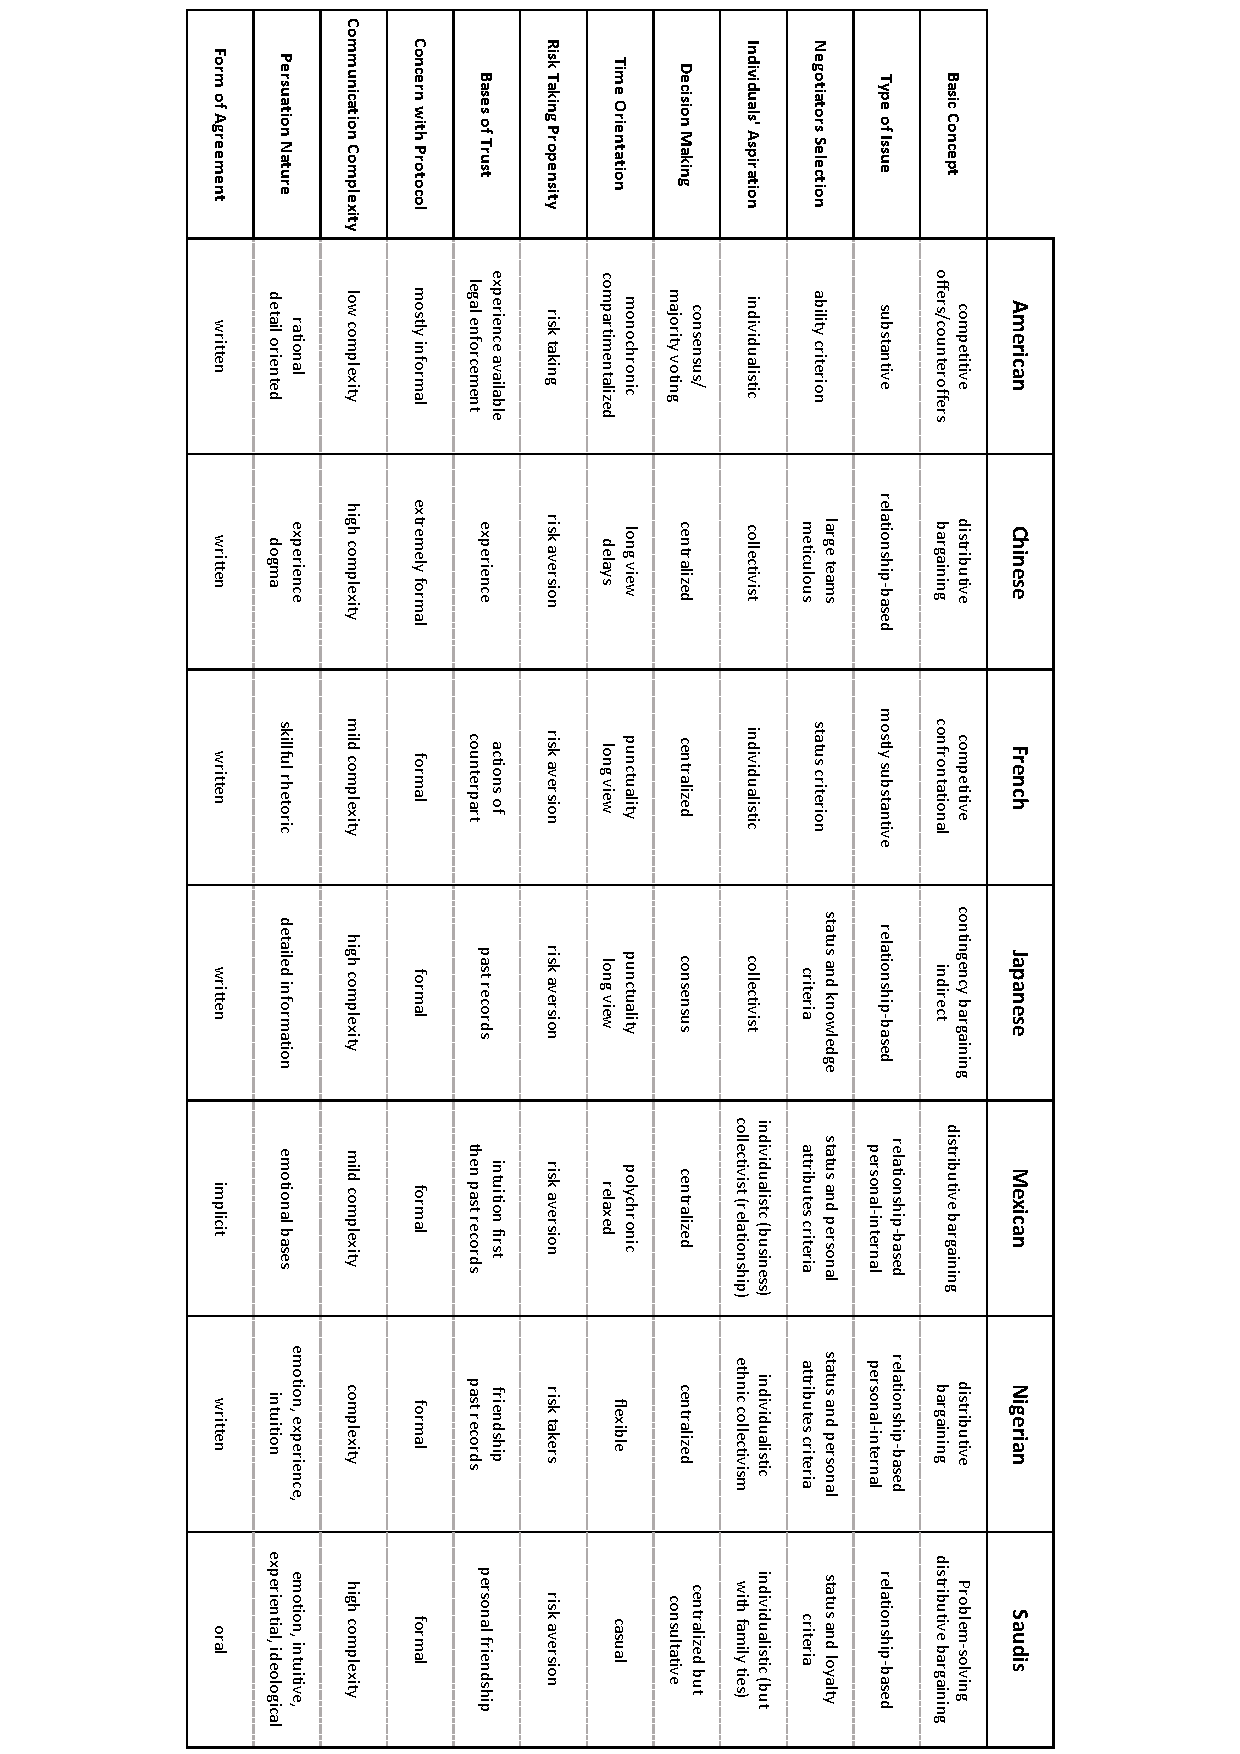
\includegraphics[totalheight=0.9\textheight, angle=180, origin=c]{images/faureTable.pdf}
%    \caption{This table shows the results of the survey: for each variable it is possible to consider the answers of each country.}%inserire caption
%    \label{faureTable}
%\end{figure}

%\noindent%
\begin{minipage}{\linewidth}% to keep image and caption on one page
    \makebox[\linewidth]{ 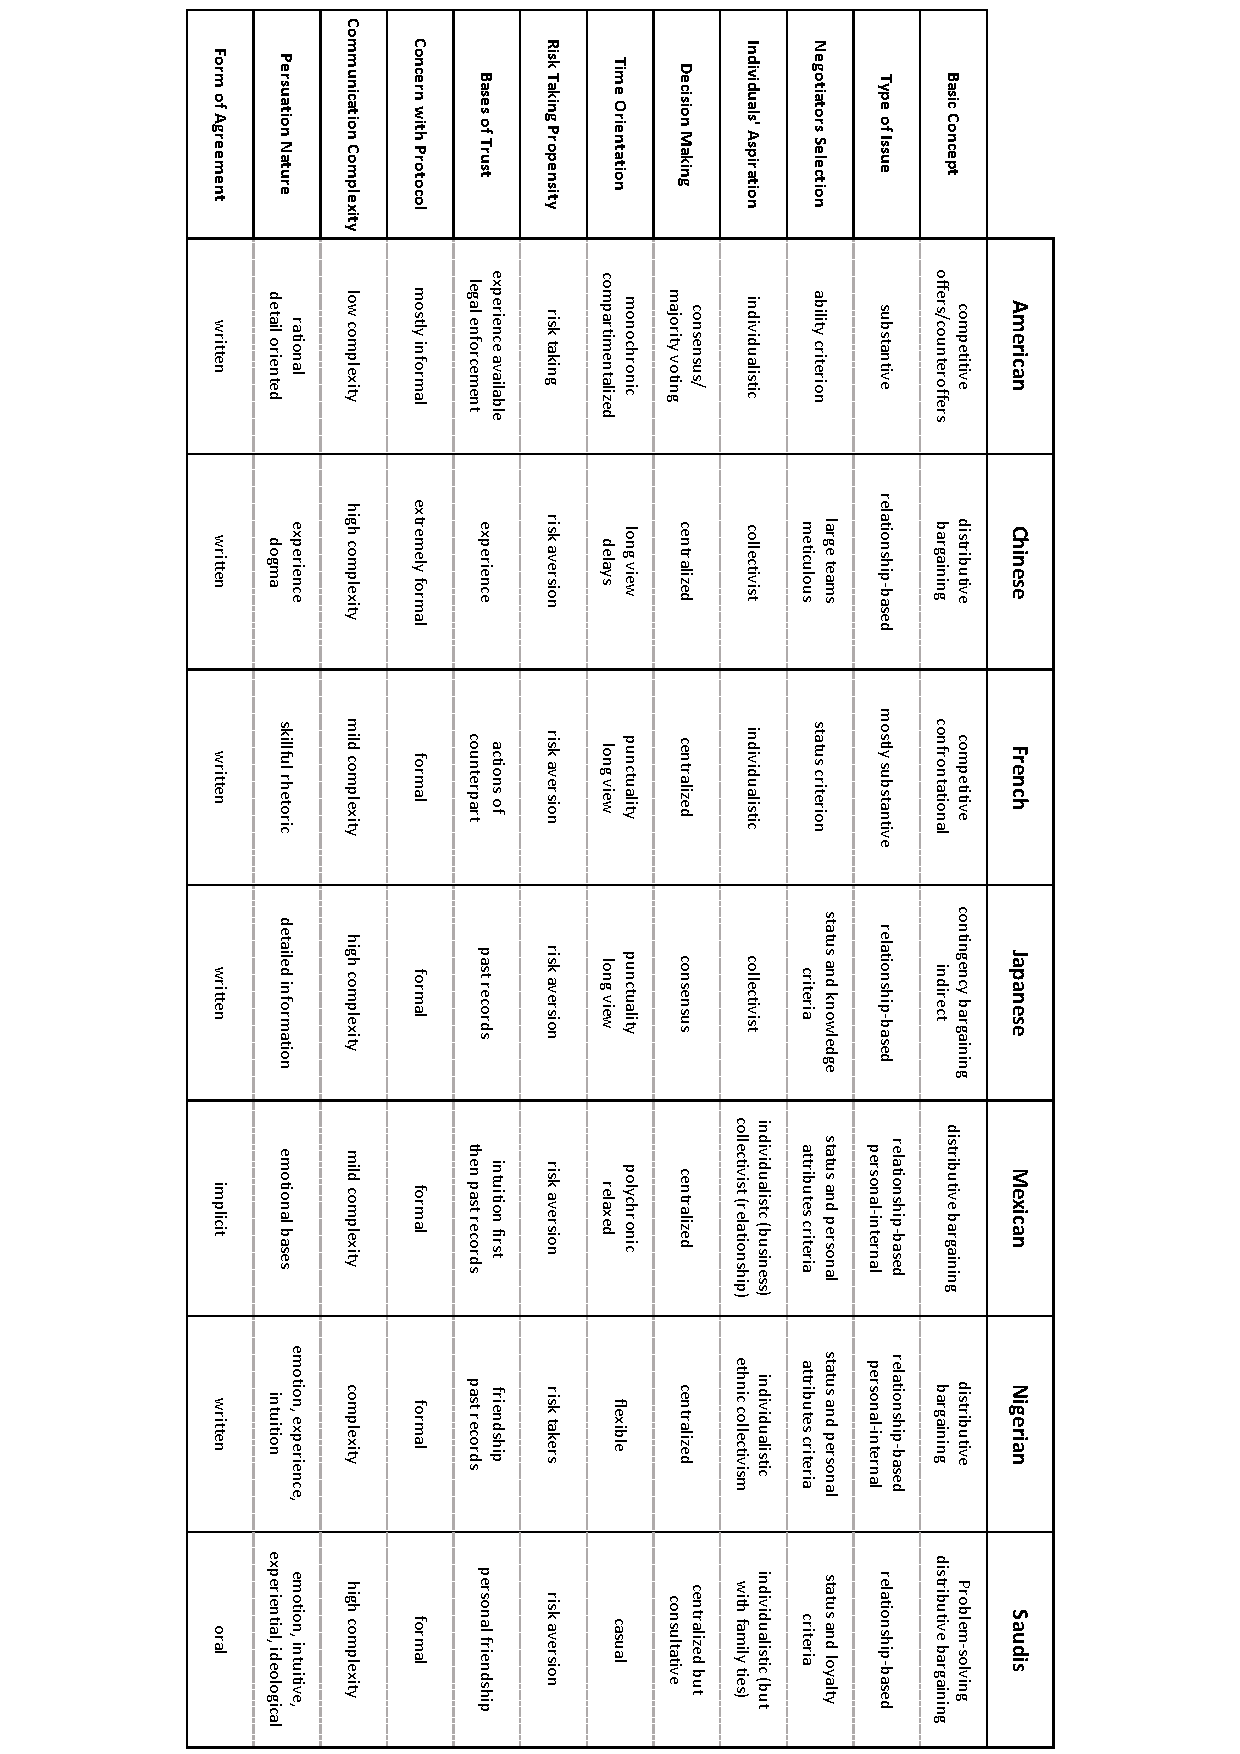
\includegraphics[keepaspectratio=true, scale = 0.7, angle=180, origin=c]{images/faureTable.pdf} }
    \captionof{figure}{This table shows the results of the survey: for each variable it is possible to consider the answers of each country.}
    \label{faureTable}
\end{minipage}

\pagebreak
Faure also cite one of his articles concerning the cognitive-strategic approach. Particularly, he cites “Negotiation: the Chinese Concept”(1998)\cite{faure1} to provide an example of a single negotiator profile. Indeed, in this article, he analyses how Chinese people conceive negotiation and how this affects the way in which they negotiate. Faure's approach is empirical and in order to assess his questions, he collected data from interviews with Chinese and Western negotiators and from live negotiations in which he was involved mainly as an observer. As already said in the previous pages, Chinese negotiation approach is mostly distributive bargaining with integrative aspects (Weiss and Stripp 1985: 12). Faure arrived to the conclusion that Chinese negotiation conception combines two different types of activities: mobile warfare and joint quest (Faure 140).

\textbf{Mobile Warfare.} Since a negotiation is conceived in a context of conflicting interests, the counterpart is sees as an adversary. Therefore, the goal is to annihilate the other party. In order to do so, many strategies can be implemented. One is to ensure to have charge of the ground. Indeed, by hosting the negotiation within their territory, Chinese negotiators can put the foreign negotiator in a position of discomfort. For example, it is common for a foreign negotiator to work during their stay in China for the negotiation: the foreign negotiator can be put in difficult work conditions, such as having to work with no heating during winter or being misplaced in a rural isolated area where is difficult to reach the outer world, let alone their superiors.
What enhances the picture of the foreign negotiator as someone to be fought is the frequent comparison to a tiger. This is to undermine their spirit in order to raise doubts in their minds, thus decreasing their strength. Another peculiar technique to undermine the foreigner's ground is to remind them about "historical mistakes attributable to their country"(Faure 41). Also, Chinese negotiators tend to be unclear in their intentions in order to confuse the other party. Moreover, the foreigner can be put "in the corner" also by reducing their space of manoeuvre through restrictions given by customs and rituals (Faure 41).
In addition, mobile warfare provides tactics such as "harassment, destabilisation, exhaustion, and squashing"(Faure 42).
Harassment is used to overwhelm the other party by firing question after question but avoiding the central points of the negotiation.
Destabilisation can be reached, for example, when during an effortless and serene negotiation, someone suddenly goes on a rant.
Exhaustion profits the fatigue of the foreign negotiator, both physical and psychological, for example by insisting on the same point for a very long time.
Lastly, squashing refers to the tactic by which a Chinese negotiator will counteroffer at a very lower level than the foreign negotiator did in order to pretend that they have no particular interest in making an agreement.

\textbf{Joint Quest.} Chinese negotiators see a negotiation with a non-Chinese negotiator as a negotiation between a civilised person and a "barbarian". Indeed, "only the foreigner who gains familiarity with Chinese culture [...] will be considered a "civilised person" by the Chinese" (1998, 43). The point is that, according to this conception (joint quest), rather than negotiating the solution, it is necessary to negotiate the construction of the problem. This peculiar state of mind comes from Taoism. Hence, "the joint quest in negotiation requires four types of actions: observing, listening, asking, and feeling"(1998, 144). The joint quest takes time and this can make Western negotiators impatient and doubtful. Indeed, as said before, Chinese negotiators value cognition more than time itself. Also, Confucian harmony takes time because it is reached through adjustments. Moreover, only an indirect approach can sustain the search for harmony. This produces two effects: negotiations become longer and observed signals are obscured (1998, 145). The joint quest is a perpetual game in which parties try to define together the negotiations' rules (1998, 146). What makes a negotiation difficult is the divergent approach adopted by Western and Chinese negotiators: the former start from the specifics to ascend to general principles, whereas the latter do the exact opposite.

To summarise, mobile warfare is the visible part of a negotiation approach, and the joint quest is the part that can be seen by reading between the lines. Changes in the mobile warfare heavily influence the frame of the joint quest. The coexistence of these two elements is possible thanks to Taoism, which promotes the duality. Mobile warfare focuses on the tactics, the joint quest on finding a common goal. It is clear how these cultural credentials have an impact on the approach of Chinese negotiators towards the process.\\

%In John Graham work %controlla citazione
%, it is possible to acknowledge the fact that culture influences negotiations on four levels: language, non-verbal behaviours, values, and thinking and decision making \cite{graham}. 

%Obviously, the language spoken is the most evident difference in an international negotiation. It is very important, regarding this issue, to have interpreters for each language spoken by the parties in a negotiation. Alternatively, the vehicular language for international exchanges is English; however, the parties can also agree upon another language they reckon is more appropriate to use before starting the negotiations. The use of interpreters can be a tool of implementing a strategy. Because, for example, it can happen that even though a negotiator can speak English, they will use the translator to have more time for a response and to observe the facial expression of the other negotiator while the translator is reporting what they said \cite{andrew}.

%Albert Mehrabian \cite{albert}, a UCLA psychologist, analysed where meaning comes from in face-to-face interactions. He discovered that, contrarily to what one may think, the words spoken carry just the 7\% of the meaning; 38\% is provided by the paralinguistic channels, that is, tone of voice, loudness, and other aspects of how things are said. The facial expression provides a remarkable 55\% of the meaning.  

%Most Americans hold on to four specific managerial values — objectivity, competitiveness, equality, and punctuality — that seem to cause misunderstandings in international business negotiation very frequently \cite{andrew}. Indeed, Americans distinguish the problem from the people thus giving it an objective framework in order to work better on the problem. Americans are score high in the individualism scale as they are very competitive: this derives from the concept of the "self-made man" on which the American dream was based. Moreover, they consider equal the buyer and the seller position, whereas in Japanese culture, for example, the buyer always seems to have the better way out of the negotiation with the seller. Lastly, time is the most valuable thing for Americans. They are the culture that most care about timing and they cannot stand things slowing down. Indeed, other negotiators will manage time so that it will become a tactic with American negotiators. 

%In the context of thinking and decision making, it is important to underline that Western culture usually divide the issues within a negotiation so that they will face them one at a time. In this way, they can measure the success of a negotiation by the way the issues are taken care of and how the related problems are solved within the process of the negotiation. On the other hand, the Eastern cultures tend to deal with the issues all together thus making it difficult for a Western negotiator to see whether the negotiation is successful or not. To overcome this issue, they can pay attention to some details during the process of the negotiations, such as the other party asking more questions on a specific issue of the negotiation, softening of the attitudes, increase of bargaining, and use of lower-level, informal communication.

Once more, it is necessary to bring up the article written by Salacuse, "Ten Ways that Culture Affects Negotiating Style: Some Survey Results" (1998)\cite{salacuse}. It is relevant (other than providing us with some insights in defining culture, particularly in distinguishing different types of cultures) because it analyses the aspects of the negotiation process that can be influenced by culture\footnote{I decided to insert this article in this chapter because of its relevance regarding the negotiators' actions and cognition.}. Particularly, the author identifies ten factors: negotiating goals, attitudes to the negotiation process, personal styles, styles of communication, time sensitivity, emotionalism, agreement form, agreement building process, negotiating team organisation, risk taking (Salacuse 223-224). 
Each of these factors are influenced by culture to the extent that negotiators' responses can be positioned on a range. In order to get results, he made a survey of "business executives, lawyers, and graduate students (many of whom had substantial work experience) from all continents at various sites in North America, Latin America, and Europe over a period of four years" (Salacuse 224).
The nationalities involved were twelve: United States, United Kingdom, France, Germany, Spain, Mexico, Argentina, Brazil, Nigeria, India, China, and Japan. Also, even professions were considered, and results came from many professional areas: engineering, law, marketing, military, finance, diplomacy, teaching, and students.

Salacuse also informs about five caveats of his survey. First, it goes without saying that the answers given by the subject of the survey were influenced by how they saw themselves. Second, it is not culture by itself that influences negotiators' behaviours: it is necessary to take into account other factors, such as personality and expertise. Third, since the survey was held in English, each respondent answered in English, hence some of the answers could not reflect truthfully their culture. Fourth, since the topics of the survey were not defined, each point was assessed by the contestants under a subjective view. Fifth, though respondents were numerous, the sample size is still exiguous. Finally, as said in chapter two, culture and nationality do not mirror each other, however Salacuse does not make this distinction. 
The following results for each category are presented by nation and by occupational affiliation. The results are shown in percentages. For a summary overview, see Figure 19 and Figure 20.

\textbf{Negotiating Goals}. Cultures, as already mentioned, see the purpose of a negotiation differently. Negotiating goals means that the negotiator aims at either achieving a contract or at building a relationship with the other party (or something in between these extremes). American negotiators stand out for being contract oriented, while Asian cultures focus on relationship. The results are shown below.

\vspace{0.3cm}
\begin{minipage}{\linewidth}
    \makebox[\linewidth]{ 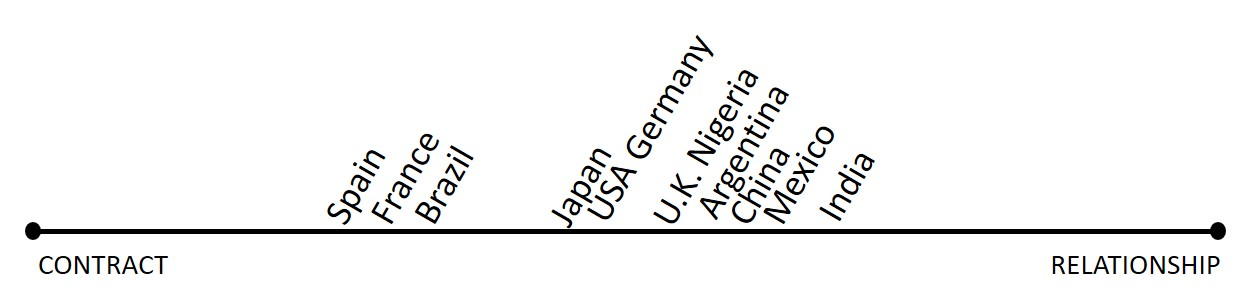
\includegraphics[width=0.65\textwidth]{images/contractSalacuse.jpg}}
    \captionof{figure}{Negotiating Goal per country.}
    \label{negotiationGoalPerCountry}
\end{minipage}
\vspace{0.3cm}

On the occupational side, it results that lawyers and military prefer contract, whereas the marketing is more inclined towards relationship.

\vspace{0.3cm}
\begin{minipage}{\linewidth}
    \makebox[\linewidth]{ 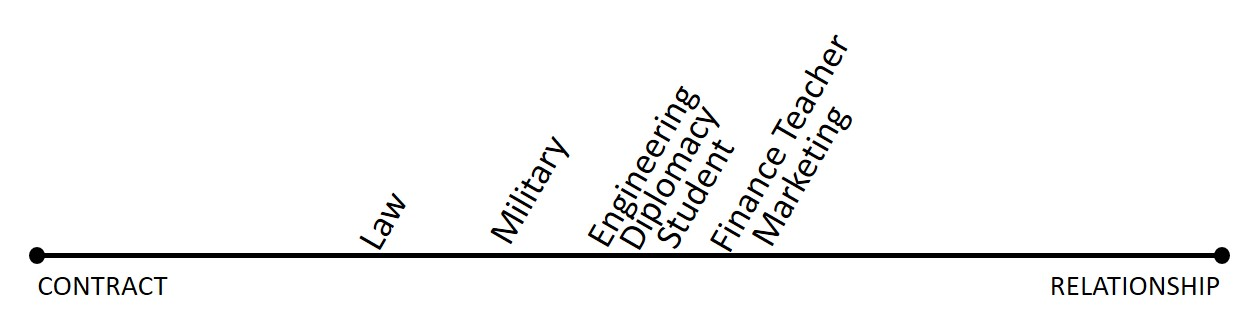
\includegraphics[width=0.65\textwidth]{images/contractprofessions.jpg}}
    \captionof{figure}{Negotiating Goal per profession.}
    \label{negotiationGoalPerProfession}
\end{minipage}
\vspace{0.3cm}

\textbf{Negotiation Attitude}. Attitudes to the negotiation process refers to the strategy adopted that can reflect a zero sum game (therefore, a win-lose situation) or a non zero sum game (meaning a win-win situation). Scholars have concluded that the former situation mirrors distributive bargaining, while the latter integrative bargaining or problem solving (1998, 227). This question highlighted a cultural difference: for example, while the entirety of Japanese respondents opted for a win-win process, though the Spanish ones were inclined for the other option.

\vspace{0.3cm}
\begin{minipage}{\linewidth}
    \makebox[\linewidth]{ 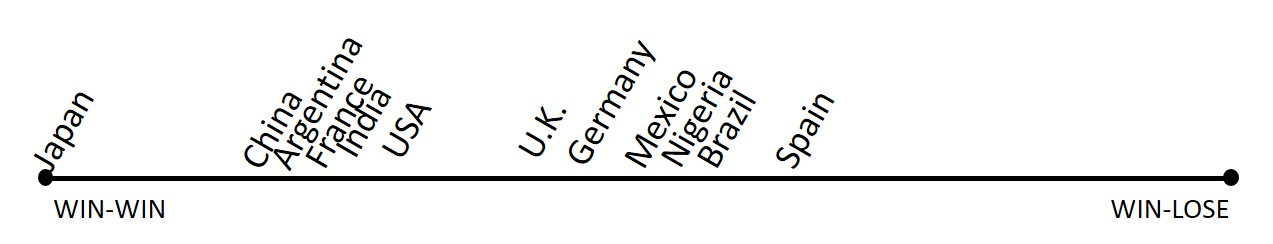
\includegraphics[width=0.65\textwidth]{images/winwin.jpg}}
    \captionof{figure}{Negotiating Attitude per country.}
    \label{negotiationAttitudePerProfession}
\end{minipage}
\vspace{0.3cm}

Concerning the professions, as expected, diplomats opt for a problem solving approach whereas the military tends to a win-lose situation.

\vspace{0.3cm}
\begin{minipage}{\linewidth}
    \makebox[\linewidth]{ 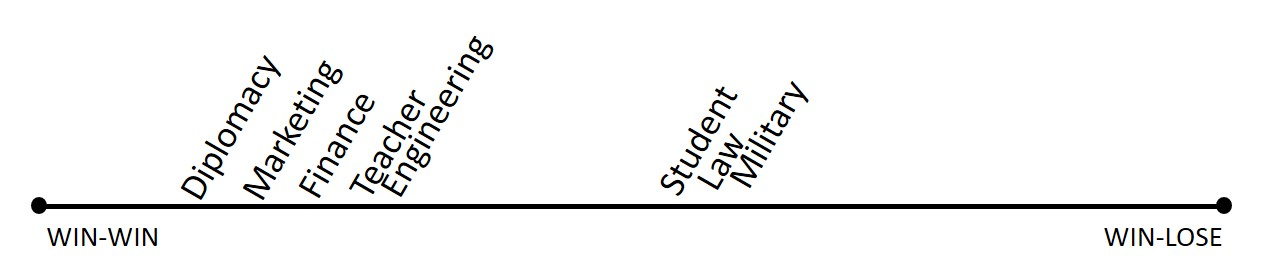
\includegraphics[width=0.65\textwidth]{images/winwinprofessions.jpg}}
    \captionof{figure}{Negotiating Attitude per profession.}
    \label{negotiationAttitudePerProfession}
\end{minipage}
\vspace{0.3cm}

\textbf{Personal Style}. Personal styles acknowledges whether the negotiator has a formal or informal approach: if the negotiator keeps addressing the respective counterpart with their titles and stays on a professional level, the negotiator is adopting a formal style; on the other hand, if the negotiator addresses the other party by their first names and tries to develop a personal connection, the negotiators is following an informal path. The majority of the interviewed declared to have an informal style, except for Nigerian people. 

\vspace{0.3cm}
\begin{minipage}{\linewidth}
    \makebox[\linewidth]{ 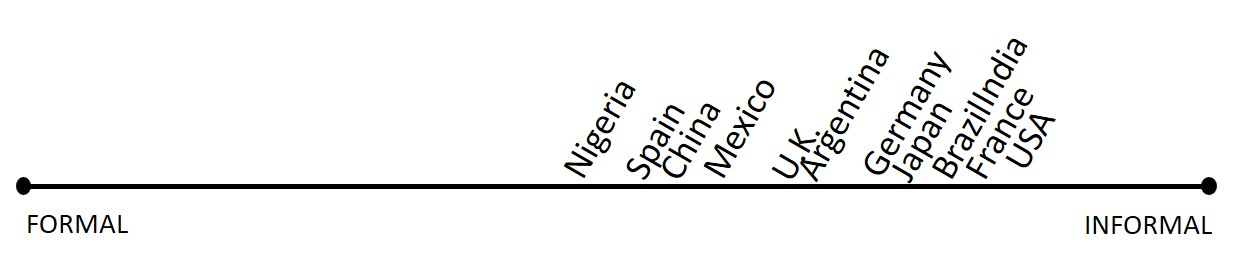
\includegraphics[width=0.65\textwidth]{images/formality.jpg}}
    \captionof{figure}{Personal Style per country.}
    \label{personalStylePerCountry}
\end{minipage}
\vspace{0.3cm}


Also under the professional partition it is possible to note some variation (1998, 229).

\vspace{0.3cm}
\begin{minipage}{\linewidth}
    \makebox[\linewidth]{ 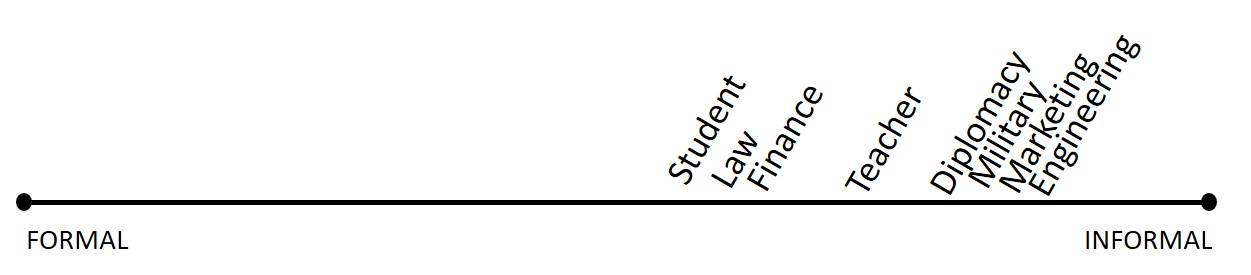
\includegraphics[width=0.65\textwidth]{images/formalprofession.jpg}}
    \captionof{figure}{Personal Style per profession.}
    \label{personalStylePerProfession}
\end{minipage}
\vspace{0.3cm}

\textbf{Communication}. A negotiator can communicate with vague allusions or figurative forms of speech (indirect style), or can deliver clear and straightforward answers (direct style). The results indicate that every participant opts for a direct form of communication. It is possible to notice that Mexico scores zero on indirect attitude, however, in the previous article, Mexican negotiators were described as people who tend to be not direct and not frank and open.

\vspace{0.3cm}
\begin{minipage}{\linewidth}
    \makebox[\linewidth]{ 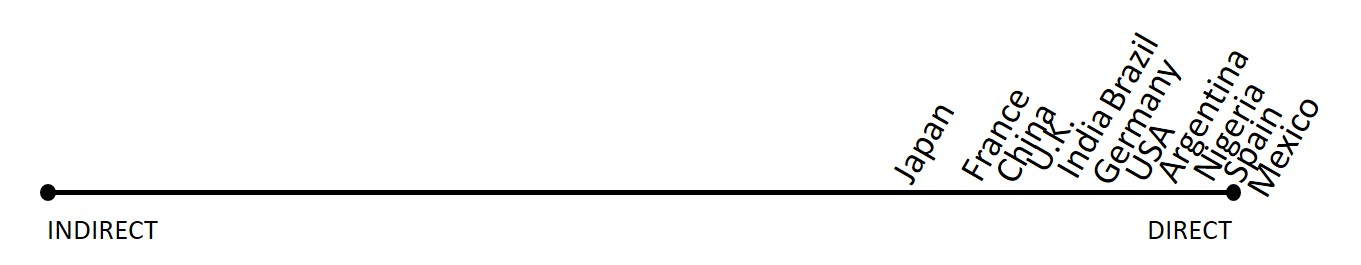
\includegraphics[width=0.65\textwidth]{images/indirect.jpg}}
    \captionof{figure}{Communication Style per country.}
    \label{communicationStylePerCountry}
\end{minipage}
\vspace{0.3cm}

Professional wise, the group that scored a higher indirect style was the diplomatic one.

\textbf{Sensitivity to time}. It refers to the punctuality in meeting a deadline or the amount of time given over to a negotiation. Almost every cultural group declared to have a high sensitivity to time, however French, Indian and German people scored a little higher than the others.

\vspace{0.3cm}
\begin{minipage}{\linewidth}
    \makebox[\linewidth]{ 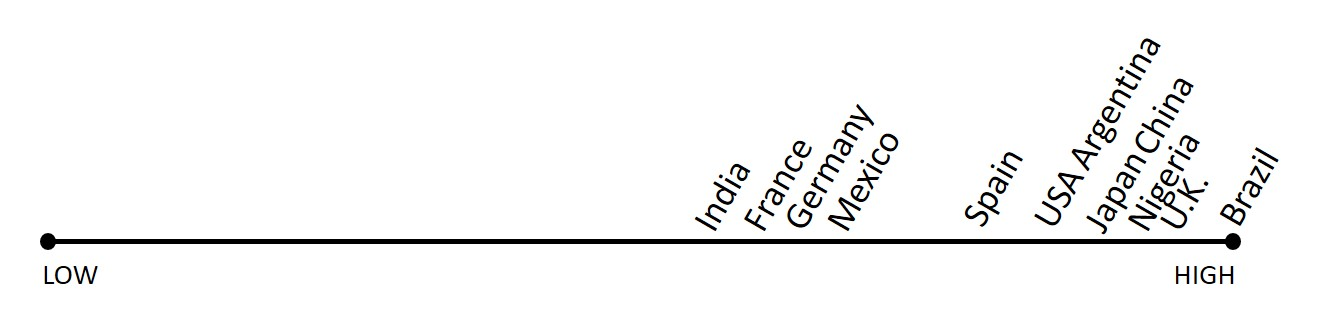
\includegraphics[width=0.65\textwidth]{images/timesensitivity.jpg}}
    \captionof{figure}{Sensitivity to Time per country.}
    \label{sensitivityTimePerCountry}
\end{minipage}
\vspace{0.3cm}

\textbf{Emotionalism}. It addresses the way a culture may display emotions, the extent to which a negotiator will demonstrate emotions is heavily influenced by culture. The responses were very various. It can be said that Latin culture scored higher in emotionalism than others.

\vspace{0.3cm}
\begin{minipage}{\linewidth}
    \makebox[\linewidth]{ 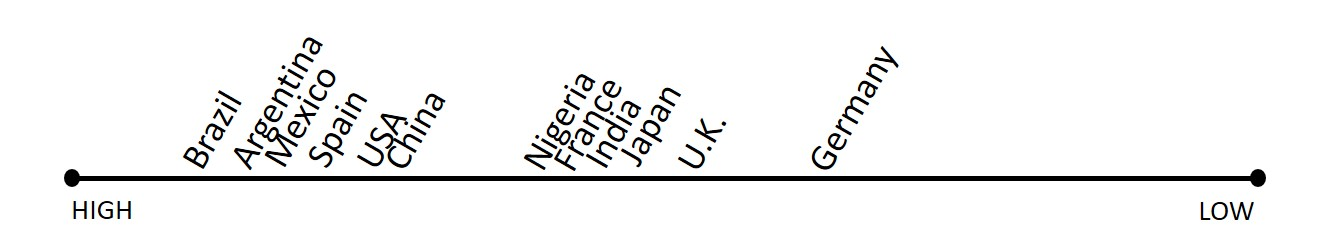
\includegraphics[width=0.65\textwidth]{images/sensitivity.jpg}}
    \captionof{figure}{Emotionalism per country.}
    \label{emotionalismPerCountry.}
\end{minipage}
\vspace{0.3cm}

\textbf{Form of Agreement}. At the end of a negotiation, parties can decide whether to have a detailed or a general agreement: culture can influence this decision. In general, results show that people tend to prefer a specific agreement instead of a general one (1998, 132). 

\vspace{0.3cm}
\begin{minipage}{\linewidth}
    \makebox[\linewidth]{ 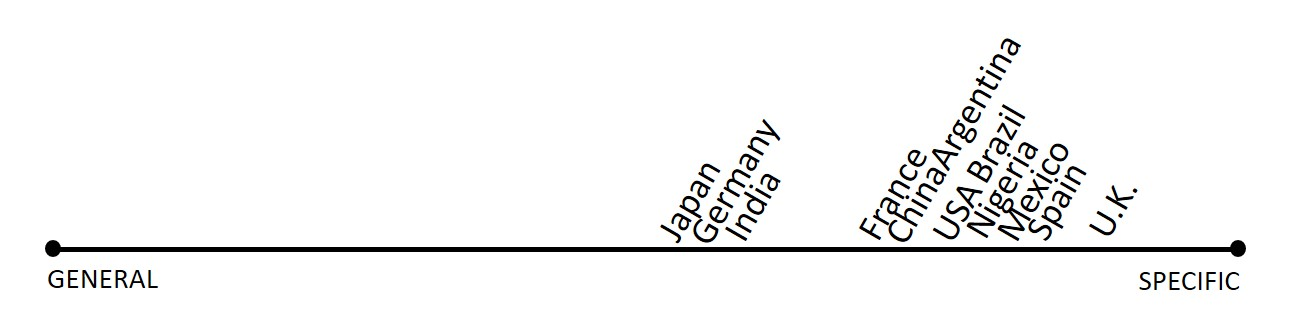
\includegraphics[width=0.65\textwidth]{images/agreement.jpg}}
    \captionof{figure}{Form of Agreement per country.}
    \label{formAgreementPerCountry}
\end{minipage}
\vspace{0.3cm}

Concerning occupations, there is a great variation among professions. On one extreme of the spectrum, there is the military, with its total propensity for a specific agreement, whereas the profession that scored the furthest from a specificity is marketing.

\vspace{0.3cm}
\begin{minipage}{\linewidth}
    \makebox[\linewidth]{ 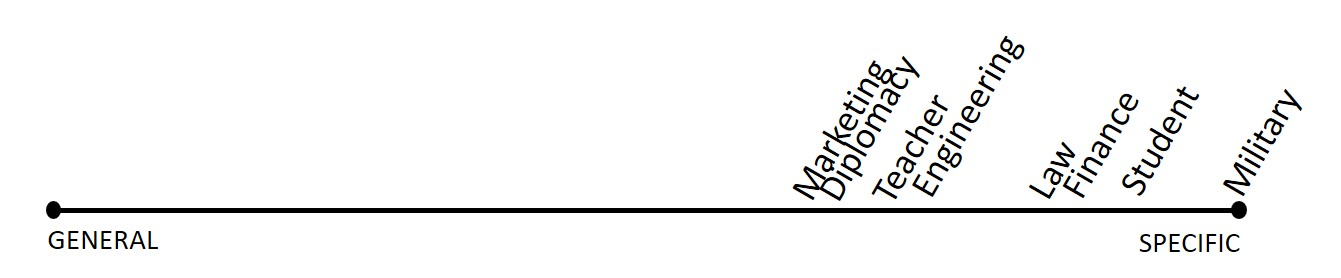
\includegraphics[width=0.65\textwidth]{images/agreementprofessions.jpg}}
    \captionof{figure}{Form of Agreement per profession.}
    \label{formAgreementPerProfession}
\end{minipage}
\vspace{0.3cm}

\textbf{Building an agreement}. Building the agreement can be done through an inductive or deductive process: the former type indicates the situation in which negotiators agree on a general principle that will give a basis on which the party can rely for the successive more specific principles; the latter implies that the negotiators will make agreements on specific details on which it will possible to extract a general principle. A deductive process is preferred by Indians, French, and Argentinians. Meanwhile, "Japanese, Mexicans and Brazilians tended to see it as a bottom-up (inductive) process" (1998, 234).

\vspace{0.3cm}
\begin{minipage}{\linewidth}
    \makebox[\linewidth]{ 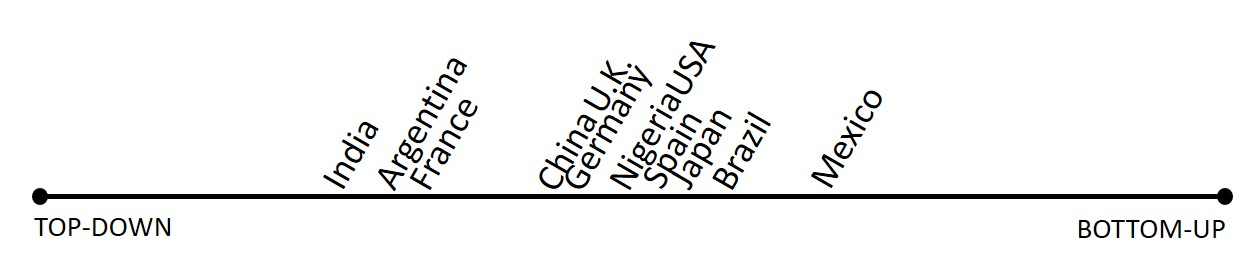
\includegraphics[width=0.65\textwidth]{images/bottomup.jpg}}
    \captionof{figure}{Building an Agreement per country.}
    \label{buildingAgreementPerCountry}
\end{minipage}
\vspace{0.3cm}

There was also variation under the professional point of view.

\vspace{0.3cm}
\begin{minipage}{\linewidth}
    \makebox[\linewidth]{ 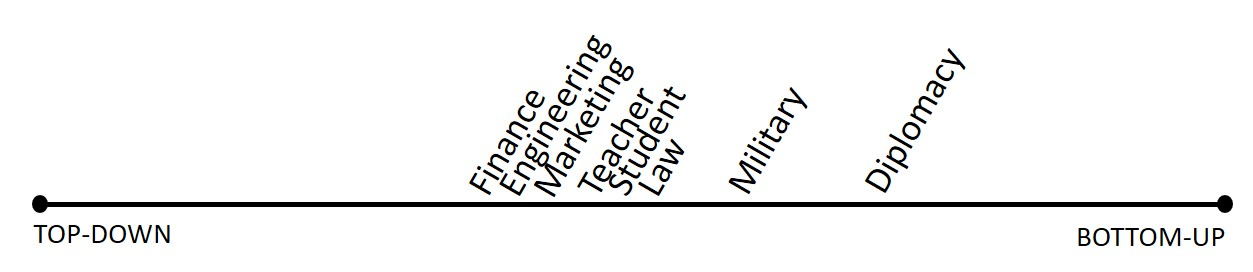
\includegraphics[width=0.65\textwidth]{images/bottomupprofessions.jpg}}
    \captionof{figure}{Building an Agreement per profession.}
    \label{buildingAgreementPerProfession}
\end{minipage}
\vspace{0.3cm}

\textbf{Team organisation}. It addresses the way organisations function: in some cultures, the focus is on the group (consensus driven approach), while in others the focus is on the individual. French scored the highest for consensus, while Brazilians, Chinese, and Mexicans opt for a one person leadership (1998, 135).

\vspace{0.3cm}
\begin{minipage}{\linewidth}
    \makebox[\linewidth]{ 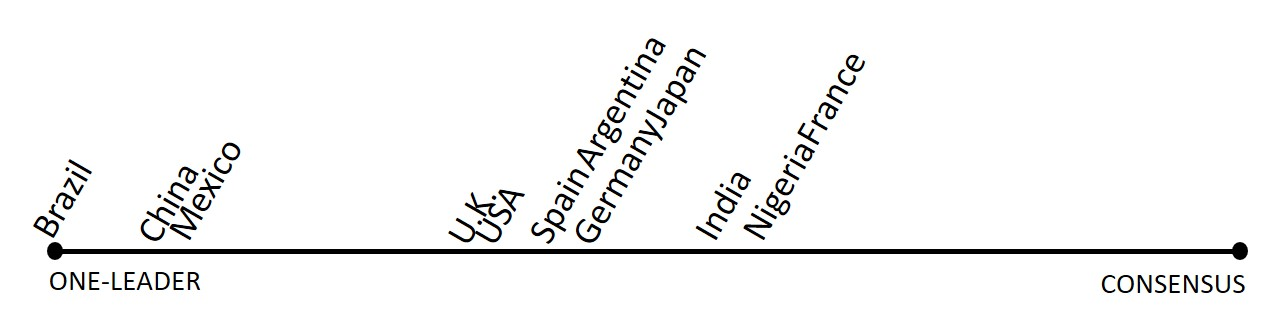
\includegraphics[width=0.65\textwidth]{images/consensus.jpg}}
    \captionof{figure}{Team Organisation per country.}
    \label{teamOrganisationPerCountry}
\end{minipage}
\vspace{0.3cm}

Intuitively, military professionals strive for a one person leadership, while the profession which scored the most propensity for a consensus is finance.

\vspace{0.3cm}
\begin{minipage}{\linewidth}
    \makebox[\linewidth]{ 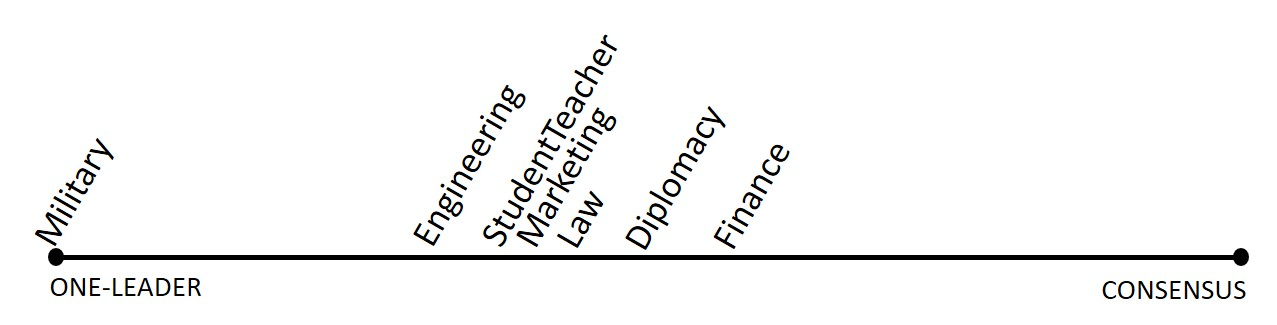
\includegraphics[width=0.65\textwidth]{images/consensusprofessions.jpg}}
    \captionof{figure}{Team Organisation per profession.}
    \label{teamOrganisationPerProfession}
\end{minipage}
\vspace{0.3cm}

\textbf{Risk Taking}. Culture can also influence the degree of risk that a negotiator is willing to take. The answers to the survey were various. The culture which showed the most aversion to risk in the Japanese one, while France scored very high in risk taking.

\vspace{0.3cm}
\begin{minipage}{\linewidth}
    \makebox[\linewidth]{ 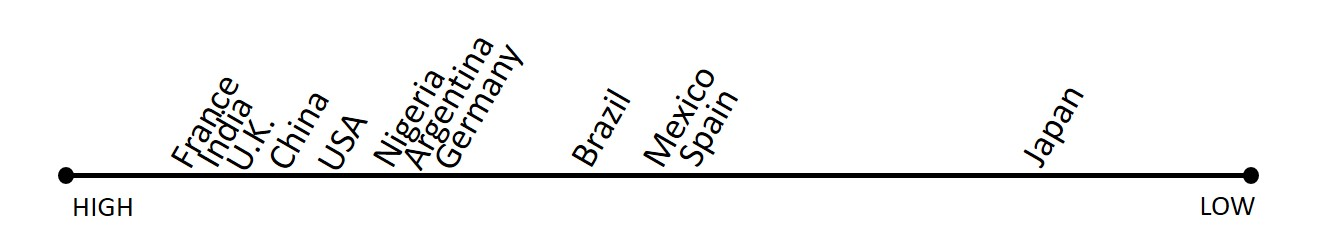
\includegraphics[width=0.65\textwidth]{images/risktaking.jpg}}
    \captionof{figure}{Risk Taking per country.}
    \label{riskTakingPerCountry}
\end{minipage}
\vspace{0.3cm}

It goes without saying that the profession who scored the highest in risk taking is the military one. The one that scored the lowest, on the other hand, is diplomacy.


\vspace{0.3cm}
\begin{minipage}{\linewidth}
    \makebox[\linewidth]{ 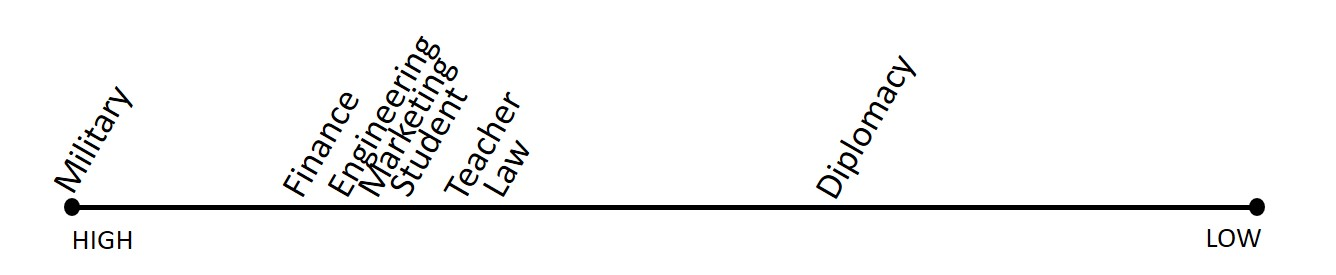
\includegraphics[width=0.65\textwidth]{images/risktakingprofessions.jpg}}
    \captionof{figure}{Risk Taking per profession.}
    \label{riskTakingPerProfession}
\end{minipage}
\vspace{0.3cm}

This article show how professional culture influences negotiators' behaviour as much as the national one.

It is possible to notice that the results of these two last articles are very similar, showing that there is a solid trend within each country. However, it is also possible to spot some inconsistencies, such as the fact that Mexicans scored zero on indirectness of communication, however, the previous article indicated Mexican negotiators as people who are not frank in their speeches and not open. This discrepancy can be justified in the fact that, as the author already specified, the answers were given directly by the participants, hence the degree of a certain variable was not uniform. Therefore, what is "direct communication" for a Mexican negotiator, might not be the same for a German or a French negotiator.

\vspace{0.3cm}
\begin{minipage}{\linewidth}
    \makebox[\linewidth]{ 
        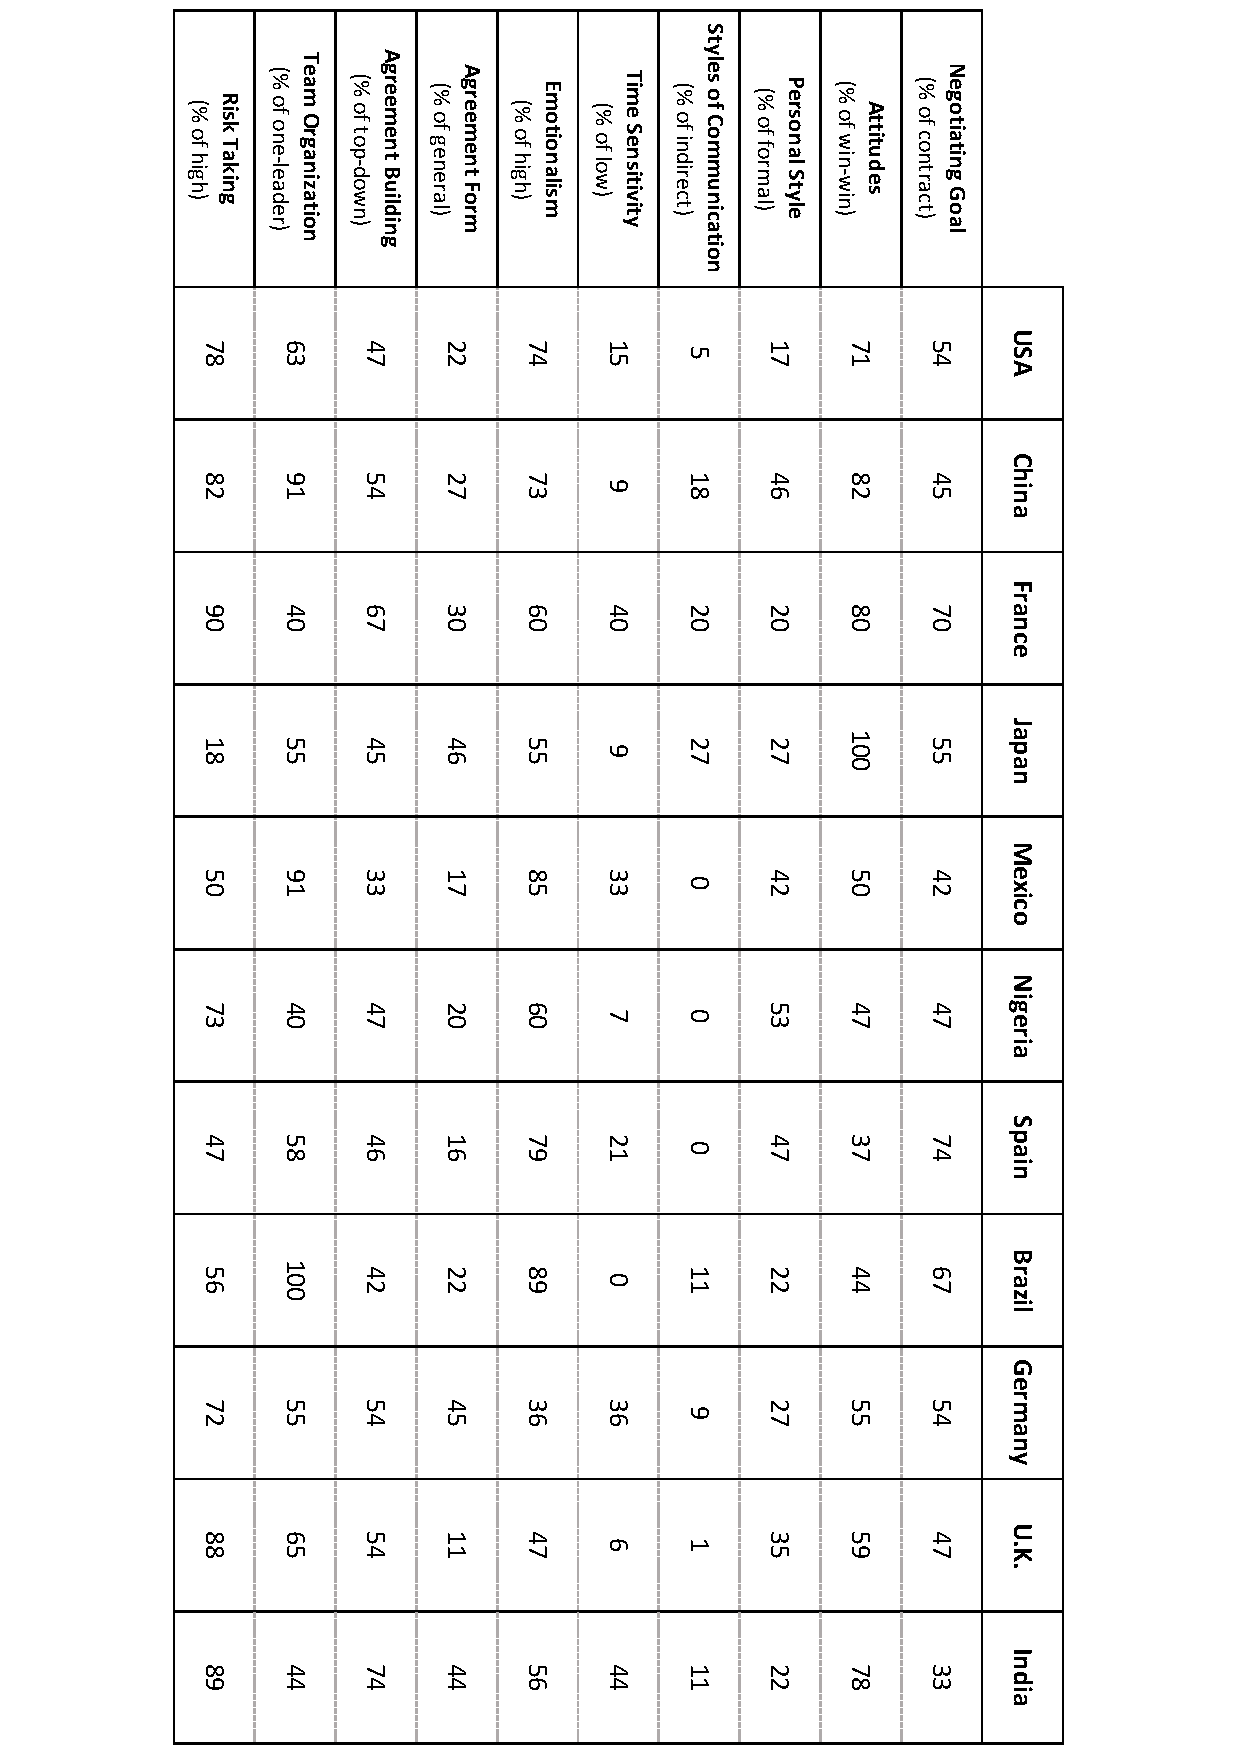
\includegraphics[keepaspectratio=true, scale = 0.5, angle=90, origin= c]{images/variablescropped.pdf}
    }
    \captionof{figure}{This table shows the results of each country considering every variable: the figures are expressed in percentage.}
\end{minipage}
\vspace{0.3cm}

\vspace{0.3cm}
\begin{minipage}{\linewidth}
     \makebox[\linewidth]{ 
        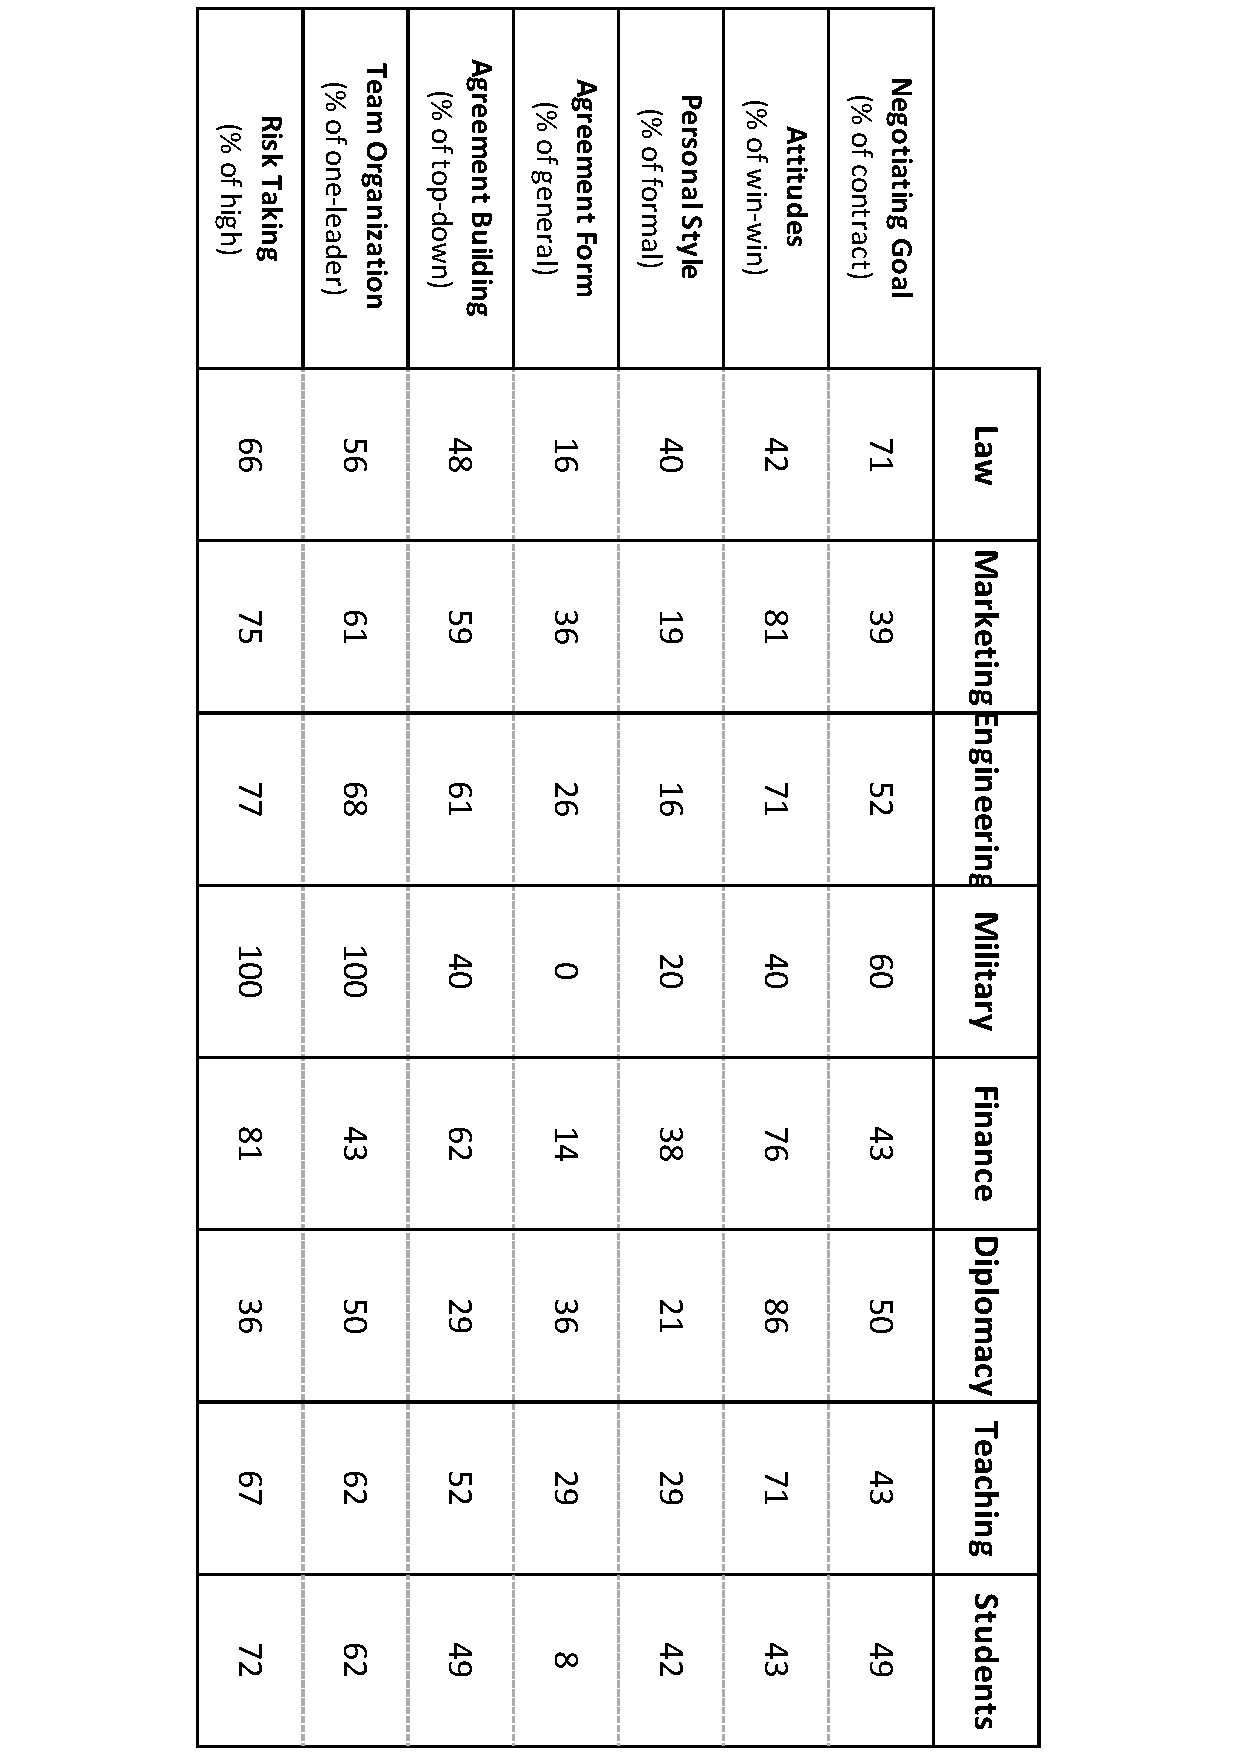
\includegraphics[keepaspectratio=true, scale = 0.5, angle=90, origin= c]{images/notvariablescropped.pdf}
    }
    \captionof{figure}{This table shows the results of each occupational field considering every variable: the figures are expressed in percentage.}
\end{minipage}
\vspace{0.3cm}

\end{document}